% discuss asympt. freedom, factorization, pdfs in "QCD and improved model"

% Then, in Access to DeltaG section, talk about scaling violation results and then pp asymmetries.

\section{QCD and the improved Parton Model}

The parton model results presented thus far assume that the photon scatters off
a free quark, a simplification which completely neglects the strong interaction.
In reality, quarks in the proton are tightly bound, constantly radiating and
reabsorbing gluons. Quantum chromodynamics (QCD) enhances the parton model with
interaction-dependent modifications of the simple parton model formulae. Two
effects are of particular interest in this work. The first is a violation of
parton density scaling; the distribution functions acquire a logarithmic
dependence on \(Q^2\) which is calculable in perturbative QCD. The second is an
anomalous gluonic contribution to \(a_0\), which at one time was thought to
offer a resolution to the ``spin crisis''. % TODO caveat about glossing over technical details, plus a citation of some review paper?

\subsection{Factorization and Scaling Violations}

\begin{figure}
  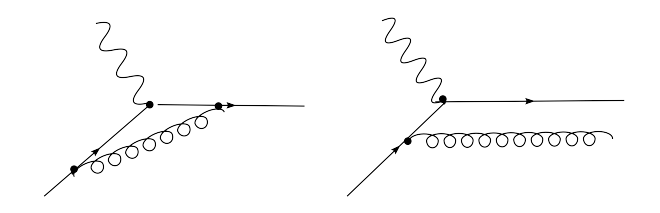
\includegraphics[width=1.0\textwidth]{figures/radiative-corrections}
  \caption{Examples of first-order radiative corrections to the quark-photon vertex.}
  \label{fig:radiative-corrections}
\end{figure}

Figure \ref{fig:radiative-corrections} illustrates two first-order gluonic
corrections to the quark-photon vertex. The diagrams contain collinear
divergences due to the massless quarks, so the size of each correction is
actually infinite. The standard technique for dealing with these infinities is
to factorize the reaction into a hard part calculable in perturbative QCD and a
soft part which must be parameterized from experimental observations. Generally
speaking, one encounters terms of the form
%
\begin{equation}
  \alpha_s~ln \frac{Q^2}{m_q^2} = \alpha_s~ln \frac{Q^2}{\mu^2} + \alpha_s~ln \frac{\mu^2}{m_q^2}.
\end{equation}
%
The first term on the right is included in the hard part of the interaction and
the second (infinite) term is absorbed into the parton distribution functions.
The factorization scale \(\mu^2\) is an arbitrary number, and exact physical
results cannot depend on it, but since perturbative results are never exact the
particular choice of scale is important. It turns out that an optimal choice is
\(\mu^2 = Q^2\), which means that perfect Bjorken scaling of the distribution
functions is broken; that is \(q(x) \rightarrow q(x,Q^2)\). However, the
dependence on \(Q^2\) is only logarithmic and is calculable by a set of
evolution equations which are presented later.

QCD factorization is completely general and not limited only to higher-order
corrections to DIS. Consider the case of mid-rapidity pion production at a high
energy proton-proton collider. The factorization theorem allows one to write the
hadronic cross section for this process as a convolution of several independent
entities: PDFs describing the probability of picking out a given parton from
each proton, a hard partonic cross section, and a fragmentation function giving
the probability that an outgoing quark will fragment into a pion with a fraction
\(z\) of the parton's momentum. To wit:
%
\begin{equation}
  \sigma_{p_A+p_B \rightarrow \pi+X} = \sum_{a,b,c} f_a(x_A, Q^2) \otimes f_b(x_B, Q^2) \otimes \sigma_{a+b \rightarrow c + X} \otimes D_c^{\pi}(z)
  \label{eqn:factorization}
\end{equation}
%
The sum is over all parton flavors that contribute to the hadronic cross
section. The \(f_i\) are the parton distribution functions; \(D_c^{\pi}(z)\) is
the pion fragmentation function for quark flavor \(c\). The partonic cross
section is calculable using perturbative QCD when the \(Q^2\) of the interaction
is large, while the PDFs and FFs must be parameterized from experimental
results. Fortunately, those distribution functions are \textit{universal}; they
can be measured in any process (commonly \(e^+e^-\) collisions) and then applied
in the calculation of any other cross section. % TODO burton has a statement about the applicability of factorization in DIS and pp->jets with 2 references here

\subsection{Anomalous gluonic contribution to $\Gamma_1$}

A particularly interesting QCD correction to DIS is shown in Figure
\ref{fig:box-diagram}. This correction involves the gluonic version of the Adler
\cite{Adler:1969gk} and Bell and Jackiw \cite{Bell:1969ts} anomalous triangle
diagram, and results in a gluonic contribution to the flavor singlet matrix
element\footnote{This result is only valid in the \(AB\) and \(JET\)
renormalization schemes. In the \(\overline{MS}\) scheme, where \(\Delta
\Sigma\) itself varies with \(Q^2\), the gluonic contribution to \(a_0\) is
zero.}:
%
\begin{equation}
  a_0(Q^2) = \Delta \Sigma_q - 3\frac{\alpha_s(Q^2)}{2\pi} \Delta G(Q^2)
  \label{eqn:qcd-a0}
\end{equation}
%
This result invalidates the simple parton model formula \ref{eqn:su3-dis} for
\(a_0\) in terms of the quark spins. In the QCD enhanced parton model, a small
measured value of \(\Gamma_1^p\) (and thus a small \(a_0\)) does not necessarily
imply small quark polarization in the proton.

\begin{figure}
  \centering
  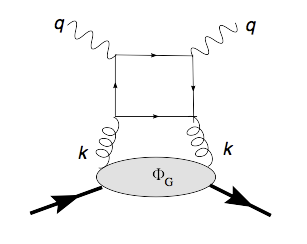
\includegraphics[width=0.5\textwidth]{figures/box-diagram}
  \caption{QCD diagram leading to the anomalous gluon contribution}
  \label{fig:box-diagram}
\end{figure}

\subsection{Spin Sum Rules}

The formulation in \ref{eqn:qcd-a0} has the attractive property that \(\Delta \Sigma_q\) is independent of \(Q^2\) and can be thought of as the quark helicity contribution even in the static (\(Q^2 \rightarrow 0\)) limit. Working in the light-cone gauge, one can write a sum rule for the proton spin which takes the form \cite{Hagler:1998kg, Harindranath:1998ve, Bashinsky:1998if}
%
\begin{equation}
  \frac{1}{2} = \frac{1}{2}\Delta \Sigma_q + \Delta G + L_q + L_g.
  \label{eqn:jaffe-sum-rule}
\end{equation}
%
Unfortunately, the last two terms are not experimentally accessible.  Lattice QCD can measure angular momentum contributions to the proton spin, but it does so in a different gauge and the sum rule \ref{eqn:jaffe-sum-rule} is not gauge invariant.

There exists an alternative sum rule \cite{Jaffe1990509, Ji:1996ek}
%
\begin{equation}
  \frac{1}{2} = \frac{1}{2}\Delta \Sigma_q + \hat{L}_q + \hat{J}_g
\end{equation}
%
where \(\hat{L}_q\) and \(\hat{J}_g\) correspond roughly to the orbital angular momentum of quarks and the total angular momentum of gluons in the nucleon. \(\hat{J}_q = \frac{1}{2}\Delta \Sigma + \hat{L}_q\) is measurable using deeply virtual Compton scattering. \(\hat{J}_g\) can then in principle be obtained through the evolution of \(\hat{J}_q\), although no experiment in the foreseeable future will provide sufficient data for that enterprise.

[End the subsection on a happier note; theorists may not have a perfectly clean model for decomposing the spin of the proton into experimental observables, but the just means experiments need to lead the way.  Or something like that.]